\documentclass[11pt, a4paper, ngerman]{arbeitsblatt}

\ladeModule{theme,boxen}

\ladeFach[datenbanken]{informatik}

\aboptionen{
	name		= {J. Neugebauer},
	kuerzel 	= {Ngb},
	titel 		= {Prüfungsvorbereitung},
	reihe 		= {Relationale Datenbanken},
	fach 		= {Informatik},
	kurs 		= {Q2},
	nummer 		= {IV.10},
	lizenz 		= {cc-by-nc-sa-eu-4},
	version 	= {2022-05-05},
}

\begin{document}
\ReiheTitel

\begin{aufgabe}[subtitle=Entity-Relationship-Modell]
	Entwirf ein Entity-Relationship-Modell zu einem Ausschnitt der Anwendung \programm{Microsoft Teams}. Öffne dazu die Teams-App und studiere die Oberfläche. Welche Elemente sind Entitäten? Wie stehen diese in Beziehung zueinander?

	Entwirf ein ER-Diagramm mit mindestens vier Entitäten und Beziehungen zwischen diesen.
\end{aufgabe}

\begin{aufgabe}[subtitle=Relationenschema]
	\begin{center}
		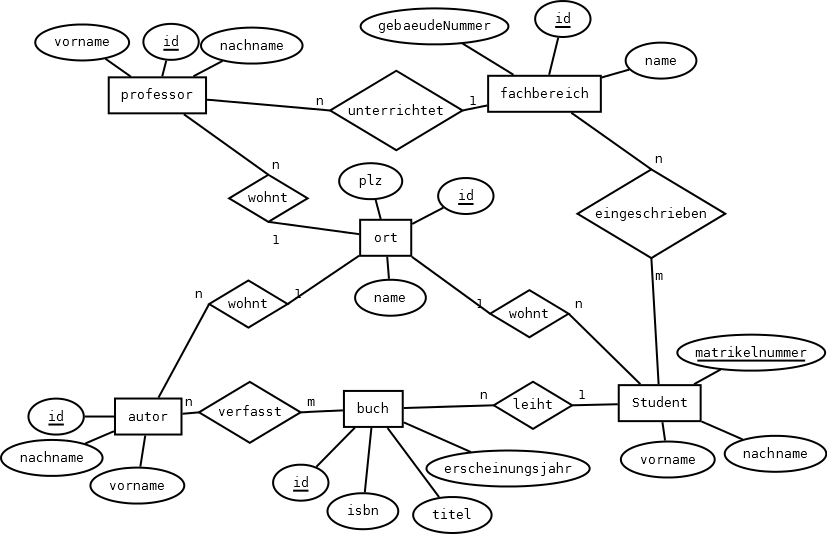
\includegraphics[width=.8\linewidth]{Q2-AB.IV.10-Abb_ERM.png}
	\end{center}

	Überführe das ER-Modell in ein Relationenschema.
\end{aufgabe}/au

\begin{aufgabe}[subtitle=Relationenschema]
	\begin{rahmen}
	\begin{smalldescr}
		\item[Fahrraeder] (\primarykey{Fahrrad\_ID}, Typbezeichnung, \foreignkey{Gangschaltung}, Farbe)
		\item[Hersteller] (\primarykey{Hersteller\_ID}, Name, \foreignkey{Ort\_Postleitzahl})
		\item[Orte] (\primarykey{Postleitzahl}, Name, Bundesland)
		\item[Gangschaltungen] (\primarykey{ID}, Name, AnzahlGaenge, Typ, \foreignkey{Hersteller})
		\item[SonstigeKomponenten] (\primarykey{ID}, Name, \foreignkey{Hersteller})
		\item[KomponentenAnFahrraedern] (\fpkey{Komponenten\_ID}, \fpkey{Fahrrad\_ID})
	\end{smalldescr}
	\end{rahmen}

	Überführe das Relationenschema in ein Entity-Relationship-Diagramm.
\end{aufgabe}

\end{document}
